\section{Introduzione}
\subsection{Scopo del documento}
Lo scopo del seguente documento è quello di illustrare le funzionalità fornite dall’applicazione e le
istruzioni per l’utilizzo della stessa. L’utente sarà quindi a conoscenza dei requisiti minimi necessari
per il corretto funzionamento di Showroom 3D.
\subsection{Glossario}
In questo documento sono state segnate con il pedice ”g” tutte le parole che, secondo noi, necessitano
di una spiegazione ulteriore per evitare eventuali ambiguità o incomprensioni. La spiegazione di questi
termini la si pu`o trovare nel documento di Glossario.
\subsection{Cos'è Showroom 3D}
Showroom 3D è un sito web che offre un'esperienza di shopping unica per gli appassionati di acquari. Grazie alla tecnologia 3D, gli utenti possono visualizzare e personalizzare in modo interattivo gli articoli per acquari come piante, rocce e decorazioni. Il sito offre una vasta gamma di prodotti di alta qualità e permette agli utenti di scegliere tra diverse opzioni di personalizzazione per soddisfare le loro esigenze. Inoltre, gli utenti possono acquistare direttamente gli articoli selezionati sul sito e riceverli comodamente a casa propria. Showroom 3D rappresenta la soluzione ideale per chi desidera rendere il proprio acquario unico e personalizzato.
\subsection{Autenticazione}
Non è presente nessuna funzione di autenticazione, quindi ogni parte e funzionalità del sito sono accessibili da chiuque senza dover effettuare un login. 
Questo perchè il progetto didattico non aveva come interesse l'unica sezione in cui sarebbe stato necessario utilizzare una pagina di autenticazione, ovvero la parte di checkout del carrello e acquisto.
\subsection{Browser supportati}
Di seguito viene fornito un breve elenco delle versioni minime di tutti i browser sui quali
il funzionamento del nostro prodotto è garantito:
\begin{itemize}
	\item Mozilla Firefox, versione 109;
	\item Google Chrome, versione 110;
	\item Micosoft Edge, versione 110;
	\item Safari, versione 16;
	\item Opera, versione 95.
\end{itemize}
Per rendere effettivo il funzionamento su tali browser, deve essere abilitato JavaScript.
\pagebreak



\section{Panoramica del sito}

Il sito subito dopo esser stato aperto presenta una schermata di caricamento con una barra di progeresso che permette di monitorare il caricamento delle risorse durante l'attesa.
\begin{figure}[H]
  \renewcommand{\thefigure}{1}
  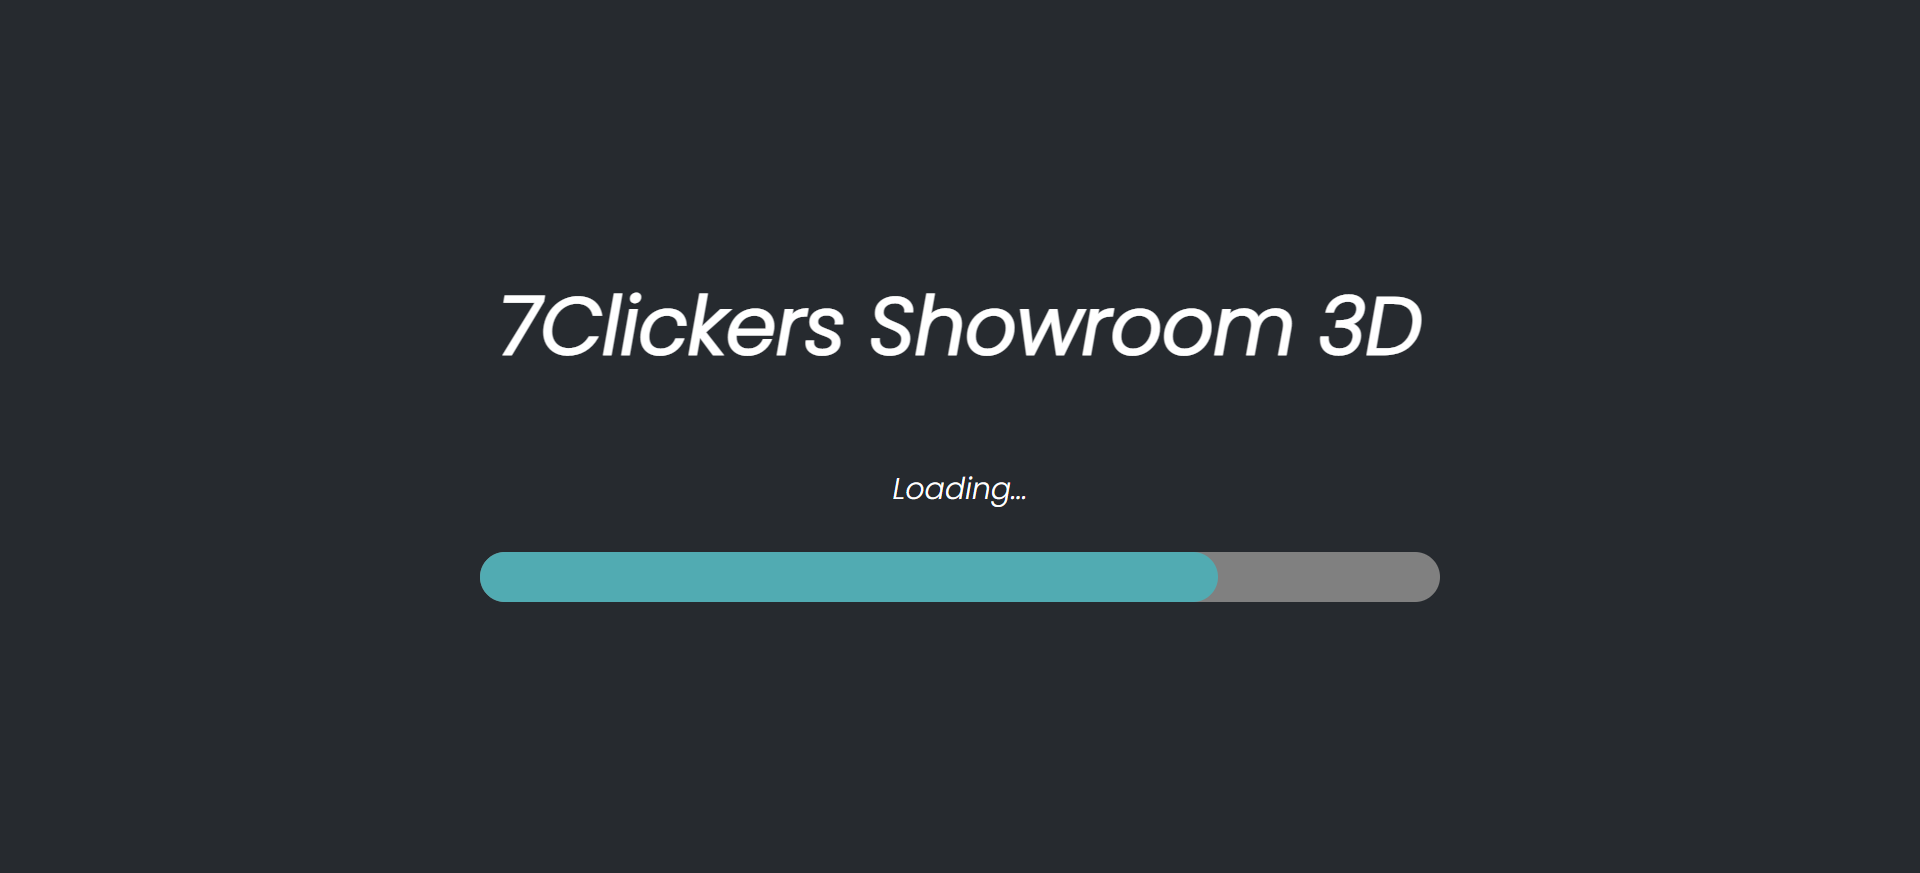
\includegraphics[width=\linewidth]{./res/images/loading_screen.png}
  \caption{Schermata di caricamento}
  \label{Schermata di caricamento}
\end{figure}
L'utente dopo il completamento del caricamento si ritrova immediatamente immerso nell'ambiente 3D, dove potrà compiere tutte le azioni e funzionalità offerte dal sito. 
\begin{figure}[H]
  \renewcommand{\thefigure}{2}
  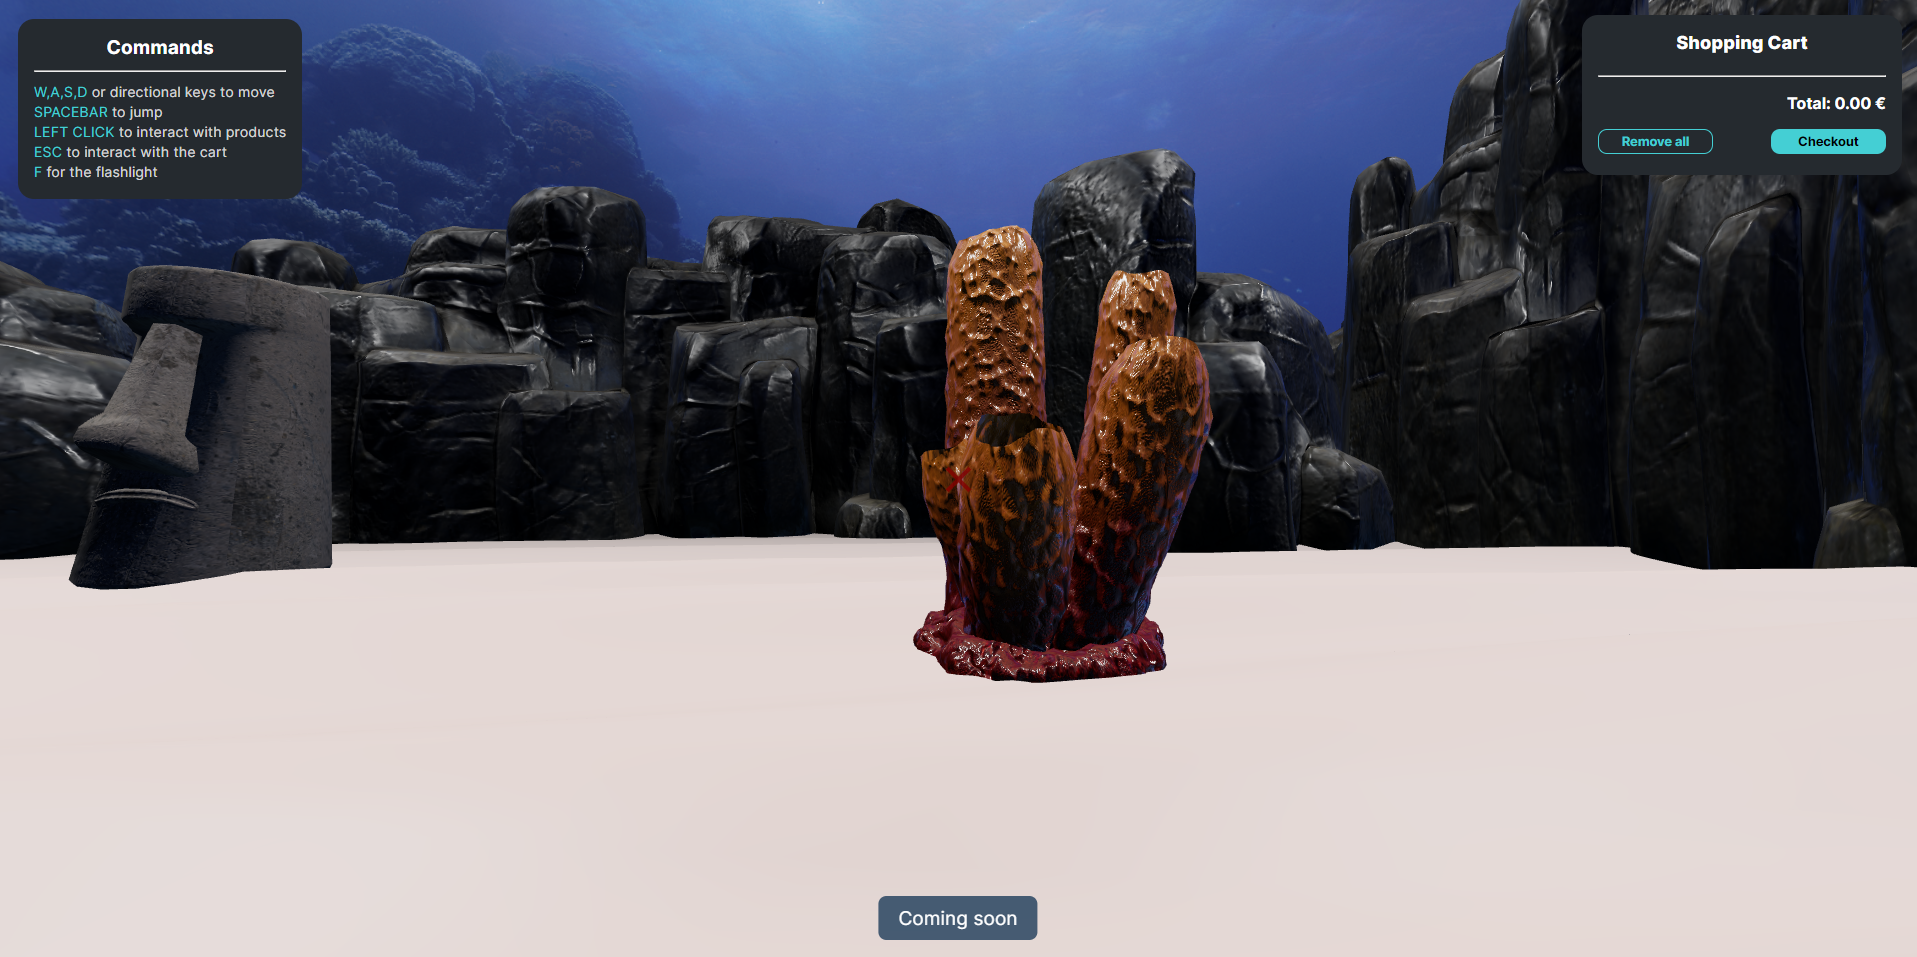
\includegraphics[width=\linewidth]{./res/images/schermata_iniziale.png}
  \caption{Showroom subito dopo l'apertura}
  \label{Showroom subito dopo l'apertura}
\end{figure}
\pagebreak

\subsection{Funzionalità}
Le funzionalità si cui può disporre l'utente sono le seguenti:
\begin{itemize}
\item navigazione in ambiente 3D immersivo;
\item visione di articoli aquistabili;
\item modifica delle caratteristiche di quest'ultimi;
\item gestione degli acquisti tramite il carrello;
\end{itemize}

\section{Interfaccia utente}
Oltre all'ambiente 3D l'utente ha a disposizioni diversi strumenti per interagire col sistema e monitorare le sue attività sul sito:
\subsection{Puntatore centrale}
Al centro della schermata è sempre presente un pallino rotondo che indica la direzione in cui sta puntando la "telecamera" dell'utente. Qunado questo pallino incrocia un elemento acquistabile nell'ambientazione comparirà a schermo il nome dell'elemento puntato e il pallino si ingrandirà leggermente e cambierà colore per notificare più chiaramente che si tratta di un oggetto con cui è possibile interagire.
\begin{figure}
  \renewcommand{\thefigure}{3}
\begin{center}
  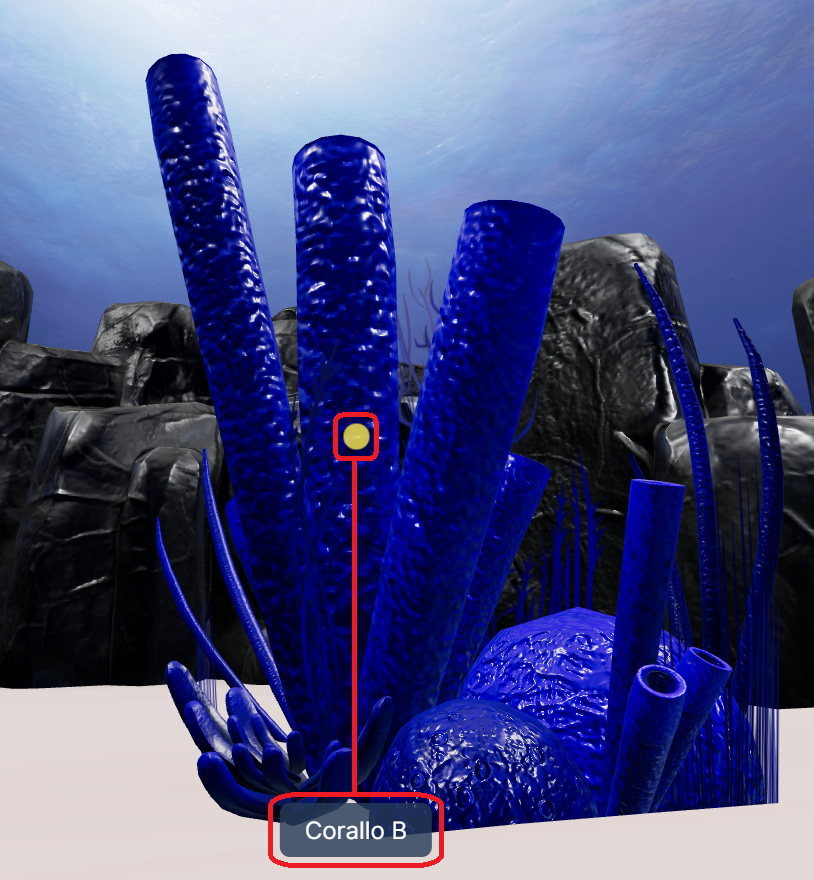
\includegraphics[width=8cm]{./res/images/puntatore.png}
 \end{center}
 \caption{Utilizzo puntatore}
  \label{Utilizzo puntatore}
\end{figure}

\subsubsection{Oggetti non interagibili}
All'interno dello showroom non tutti gli oggetti sono in vendita ed interagibili, sono anche presenti delle decorazioni che hanno il solo scopo di arricchire l'ambientazione e renderla più realistica.
Al fine di differenziare queste due tipologie di oggetti il puntatore centrale si trasformerà in una croce rossa quando punta verso un'oggetto di decorazione non interagibile, inoltre, al posto del nome dell'oggetto, in basso comparirà la scritta "coming soon".
IMMAGINE PUNTATORE A X

\pagebreak

\subsection{Item sidebar}
Clickando il tasto sinistro del mouse quando la telecamera è puntata su un'oggetto è possibile aprirne la scheda che si presenta in questo modo:
\begin{figure}[H]
  \renewcommand{\thefigure}{4}
\begin{center}
  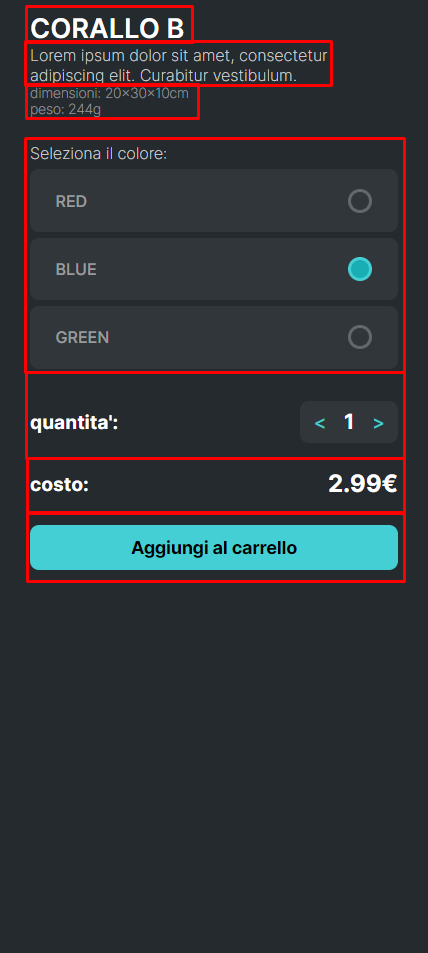
\includegraphics[width=8cm]{./res/images/scheda_evidenziata.png}
 \end{center}
 \caption{Dettagli scheda del prodotto}
  \label{Dettagli scheda del prodotto}
\end{figure}
Come si nota dall'immagine la scheda riporta molte informazioni rigurdo all'oggetto, ovvero:
\begin{itemize}
	\item Nome;
	\item Descrizione;
	\item Dimensioni;
	\item Peso;
	\item Colore;
	\item Quantità: selezionando una delle due freccie di questa riga è possibile aumentare o diminuire la quantità dell'oggetto da inserire nel carrello;
	\item Costo;
	\item Pulsante "Aggiungi al carrello": premendo questo pulsante verranno inseriti nel carrello un numero di oggetti che dipende dalla quantità selezionata e con le caratteristiche scelte.
\end{itemize}

Per chiudere la scheda dell'oggetto e tornare alla normale navigazione della stanza basta premere col mouse al di fuori di essa.
\subsubsection{Personalizzazione}
All'interno della sidebar è possibile trovare alcuni campi modificabili, identficati da una serie di pulsanti con cui l'utente può effettuare la sua personalizzazione.
Deselezionando il pulsante di modifica di una caratteristica è possibile riportare quella caratteristica alla sua versione standard.
Ogni oggetto è modificabile in almeno una caratteristica tra:
\begin{itemize}
	\item Colore;
	\item Taglia;
	\item Texture.
\end{itemize}
Una volta effettuata la modifica questa sarà applicata anche nell'ambinte 3D e sarà quindi possibile osservare l'oggetto nelle sue varie configurazioni prima di effettuare l'aquisto una queste.
\begin{figure}[H]
  \renewcommand{\thefigure}{5}
\begin{center}
  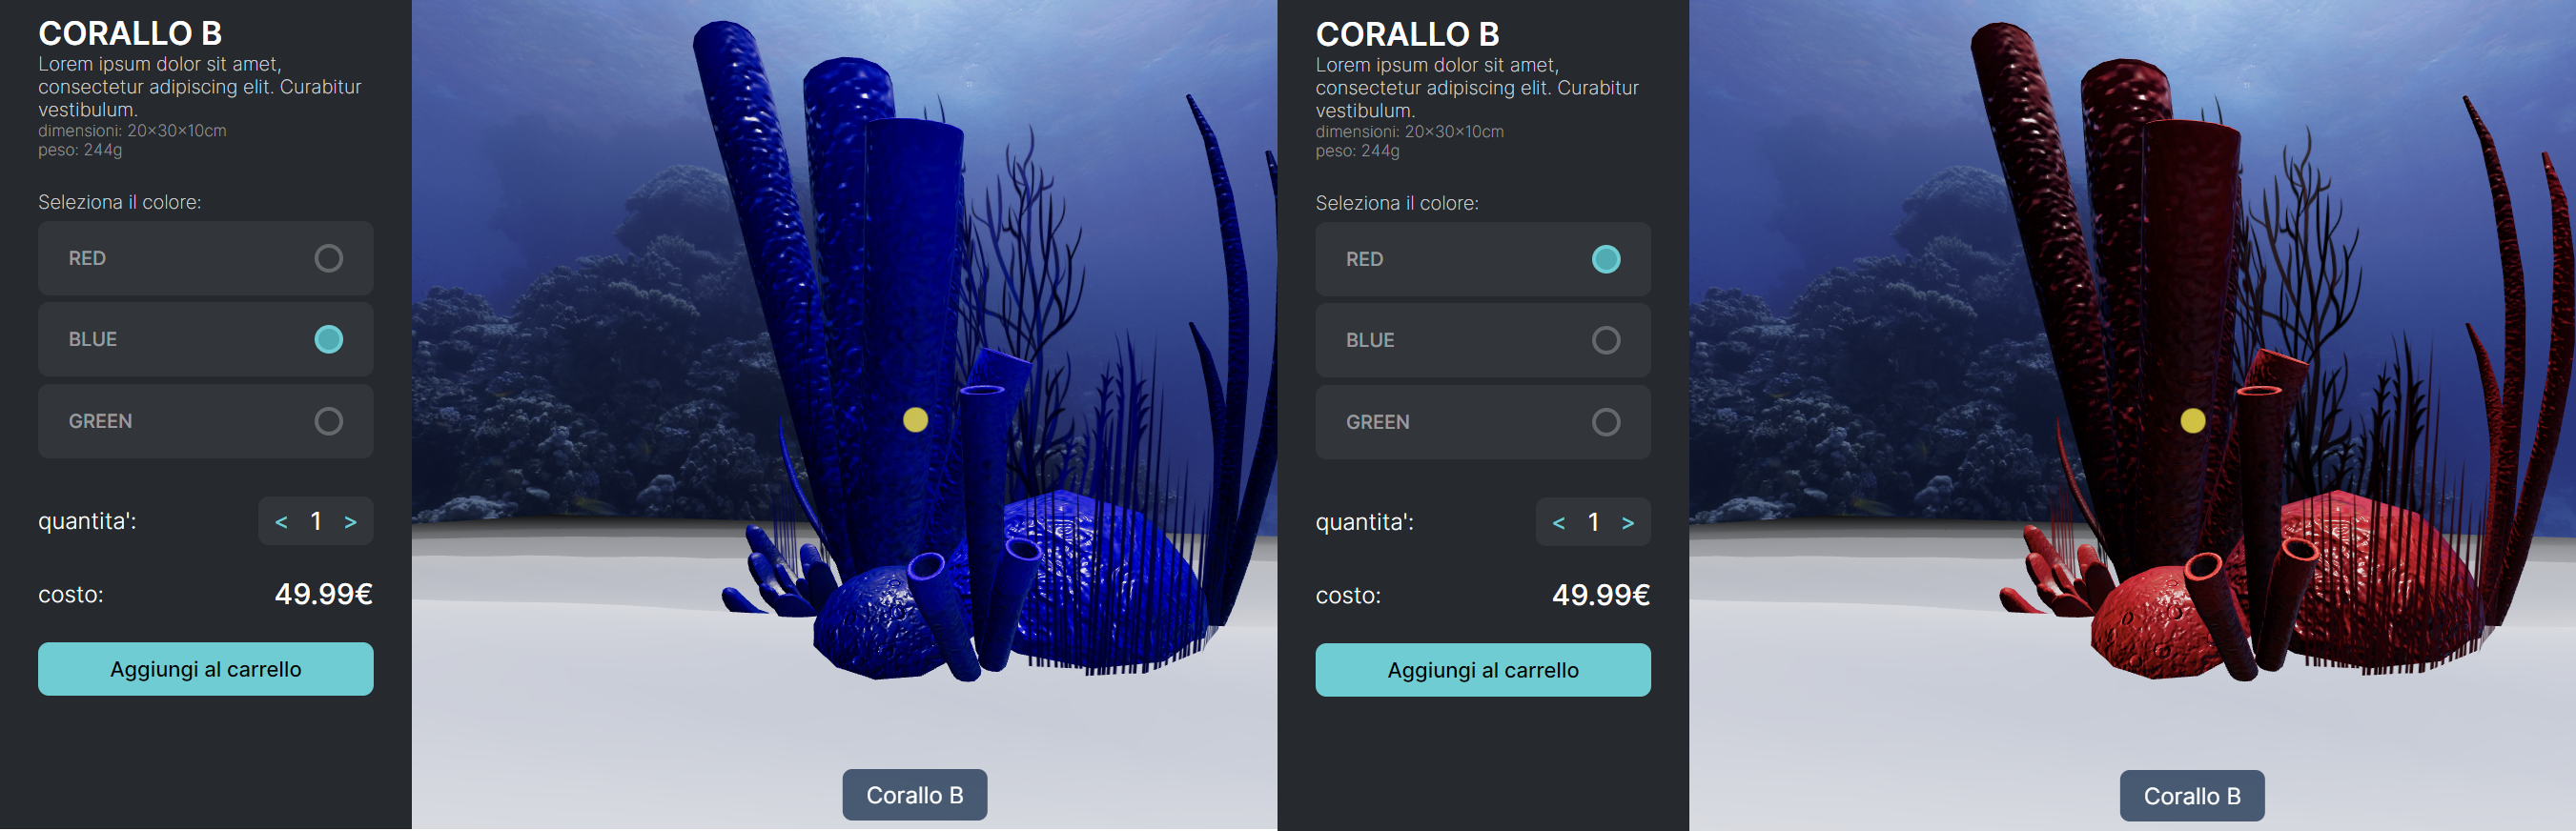
\includegraphics[width=\linewidth]{./res/images/modifica.png}
\end{center}
  \caption{Modifica colore di un oggetto}
  \label{Modifica colore di un oggetto}
\end{figure}
\pagebreak

\subsection{Carrello}
\begin{figure}[H]
  \renewcommand{\thefigure}{6}
\begin{center}
  \includegraphics[width=8cm]{./res/images/carrello.png}
\end{center}
  \caption{Carrello}
  \label{Carrello}
\end{figure}

Una volta acquistato un oggetto, quet'ultimo verrà inserito nel carrello (in basso a destra nello schermo), riportandone il nome, le caratteristiche personalizzate e il prezzo unitario.
Il carrello si presenta quindi come un elenco inizialmente vuoto, che si aggiorna in tempo reale e riporta gli oggetti scelti dal cliente.
In fondo al carrello si trovano:
\begin{itemize}
	\item Pulsante Checkout;
	\item Pulsante Svuota carrello;
	\item Prezzo totale.
\end{itemize}
Il carrello è fittizio, cioè non permette di effettuare veramente degli acquisti, infatti non è prevista nessuna funzione di pagamento ed inoltre non è persistente, cioè non salva nessun dato e tra una sessione e l'altra viene completatmente svuotato.
\pagebreak

\subsection{Illuminazione}
All'interno dello showroom è presente una luce ambientale che illumina in modo uniforme tutto l'ambiente, ma al fine di offrire una visione più dinamica dell'ambientazione e degli oggetti in vendita sono state inserite le seguenti caratteristiche:
\begin{itemize}
	\item una "nebbia" ovvero una progressiva diminuzione della luminosità mano a mano che ci si allontana da un punto.
	\item una "torcia" che proietta una luce direzionale (conica) davanti all'utente. Questa funzionalità si può attivare e disattivare premendo il pulsante F.
\end{itemize}

\begin{figure}[H]
  \renewcommand{\thefigure}{7}
  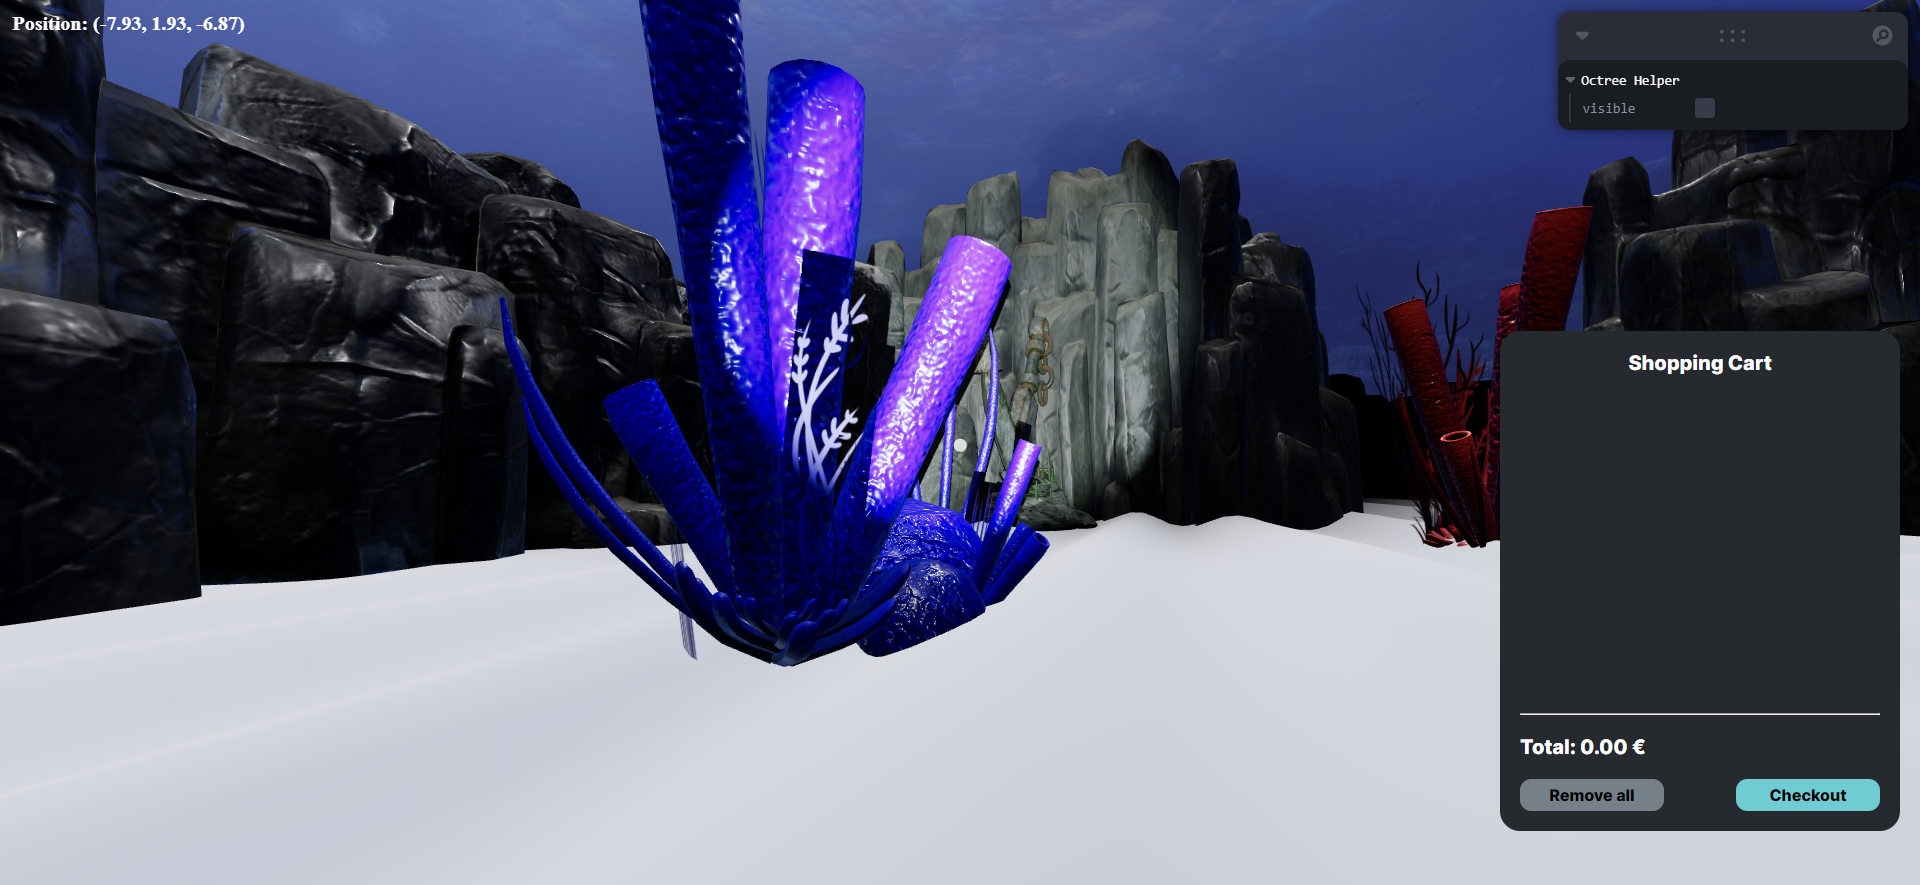
\includegraphics[width=\linewidth]{./res/images/torcia.png}
  \caption{Torcia accesa}
  \label{Torcia acccesa}
\end{figure}


\section{Navigazione}
All'interno dello showroom sono previsti varie possibilità e limiti per muoversi:
\begin{itemize}
	\item Movimento orizzaontale coi tasti ↑ (avanti) ← (sinistra) → (destra) ↓ (indietro) oppure rispettivamente coi tasti w a s d;
	\item Salto (breve movimento in alto per poi ricadere a terra) premendo la barra spaziatrice. L'altezza del salto viene limitato se si prova a salire troppo in alto, per evitare di superare i limiti della mappa;
	\item Collisioni con gli oggetti. Se l’utente prova a collidere con un oggetto il movimento viene interrotto;
	\item Collisioni con il limite della mappa. La zona in cui si muove l'utente è delimitata con vari ostacoli che fanno parte dell'ambientazione, se l'utente prova a muoversi al loro interno il movimento viene interrotto. 
	\item Nel caso in cui l'utente dovesse riuscire ad oltrepassare i limiti della stanza verrà teletrasportato al punto predefinito dal quale è iniziata la navigazione.
\end{itemize}
\begin{figure}[H]
  \renewcommand{\thefigure}{8}
  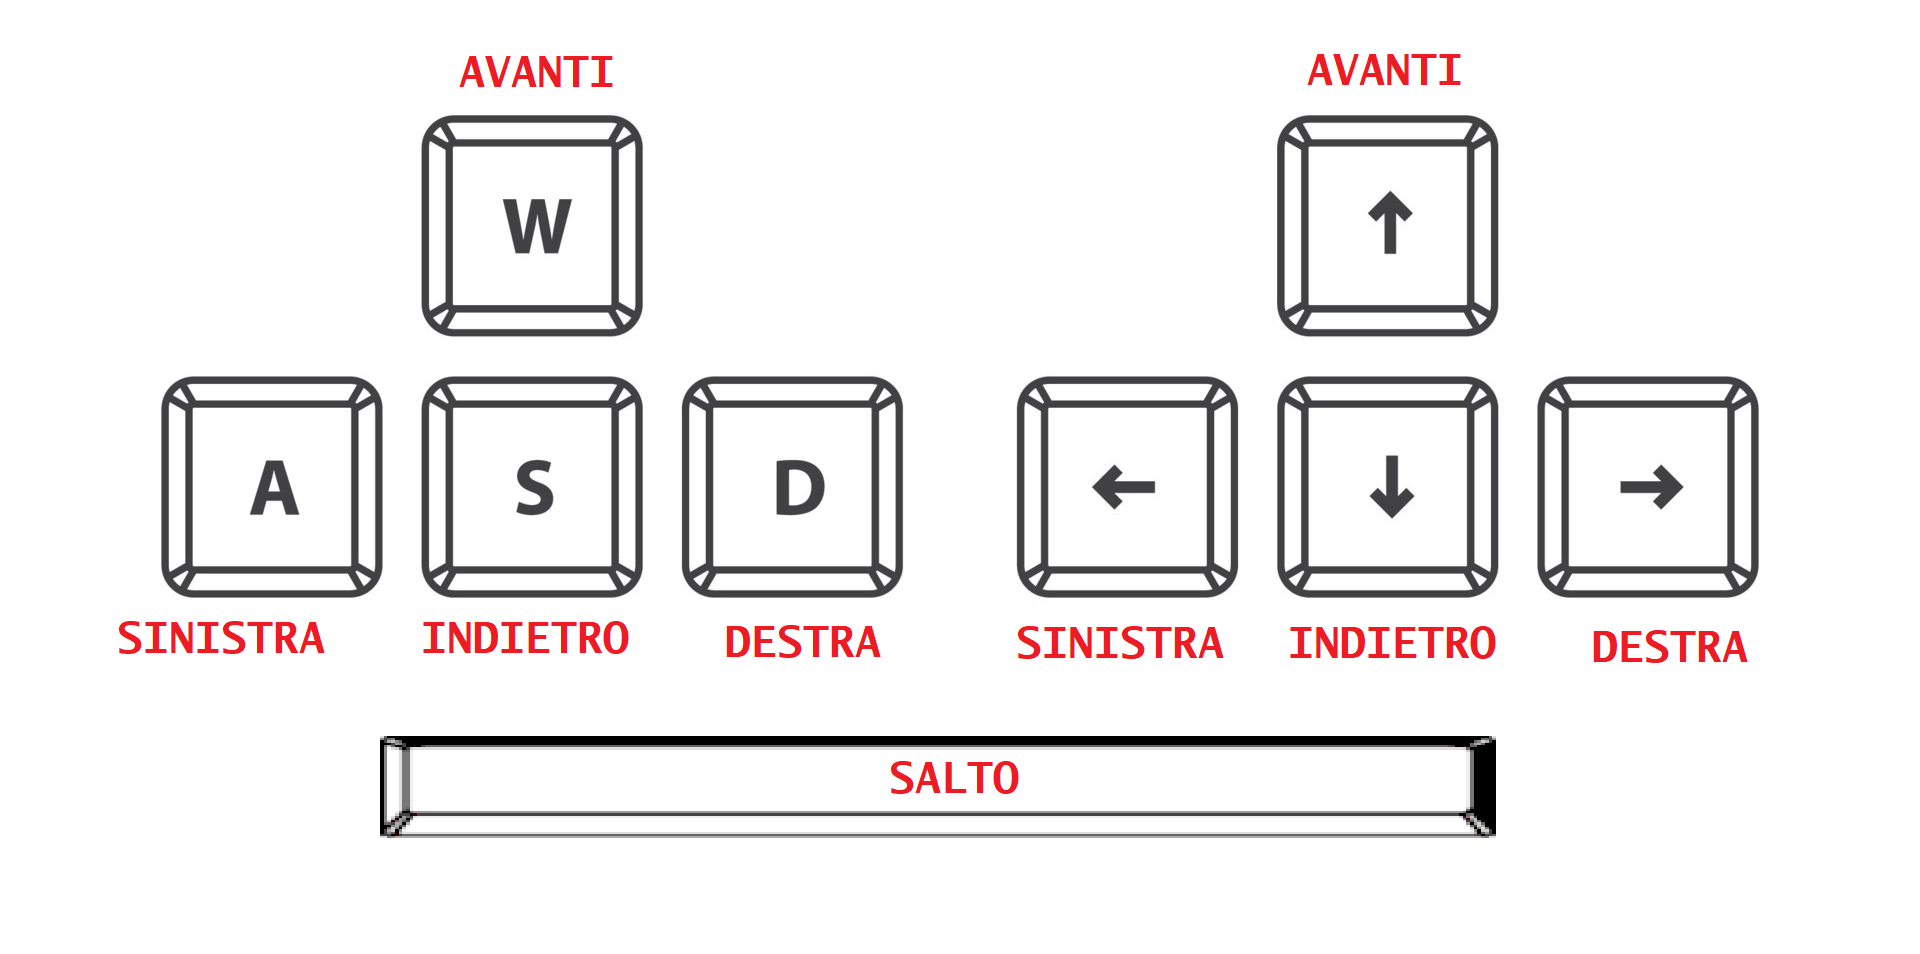
\includegraphics[width=\linewidth]{./res/images/comandi_direzionali.png}
  \caption{comandi direzionali}
  \label{comandi direzionali}
\end{figure}

\subsection{Stanze}
Lo showroom è suddiviso in due stanze, contenenti due tipologie di articoli diversi:
\begin{itemize}
	\item Tema coralli
	\item Tema pirati
\end{itemize}
In ognuna delle due stanze vengono venduti articoli inerenti al tema.\\
Le stanze sono interconnesse tra loro ed è possibile arrivare ad ogni stanza semplicemente camminando nell'ambientazione, senza quindi l'utilizzo di diversi tipi di navigazione o di cambi di pagina web.
Questo è il collegamento tra la stanza coralli e la stanza pirati
IMMAGINE TUNNEL (SONO QUESTI I TEMI DELLE DUE STANZE?)

\pagebreak


